% #############################################################################
% This is Appendix B
% !TEX root = ../main.tex
% #############################################################################
\chapter{Case Studies}
\label{appendix:appendixB}

In this appendix, we present additional information about the case studies explored in \cref{chap:evaluation}, including information about the configuration of each algorithm and the results obtained in each run. All the configurations but the ones referred in the following sections are the default configurations provided by the libraries used to develop the optimization framework.

\section{Ericeira House}

\begin{figure}[htbp]
	\centering
	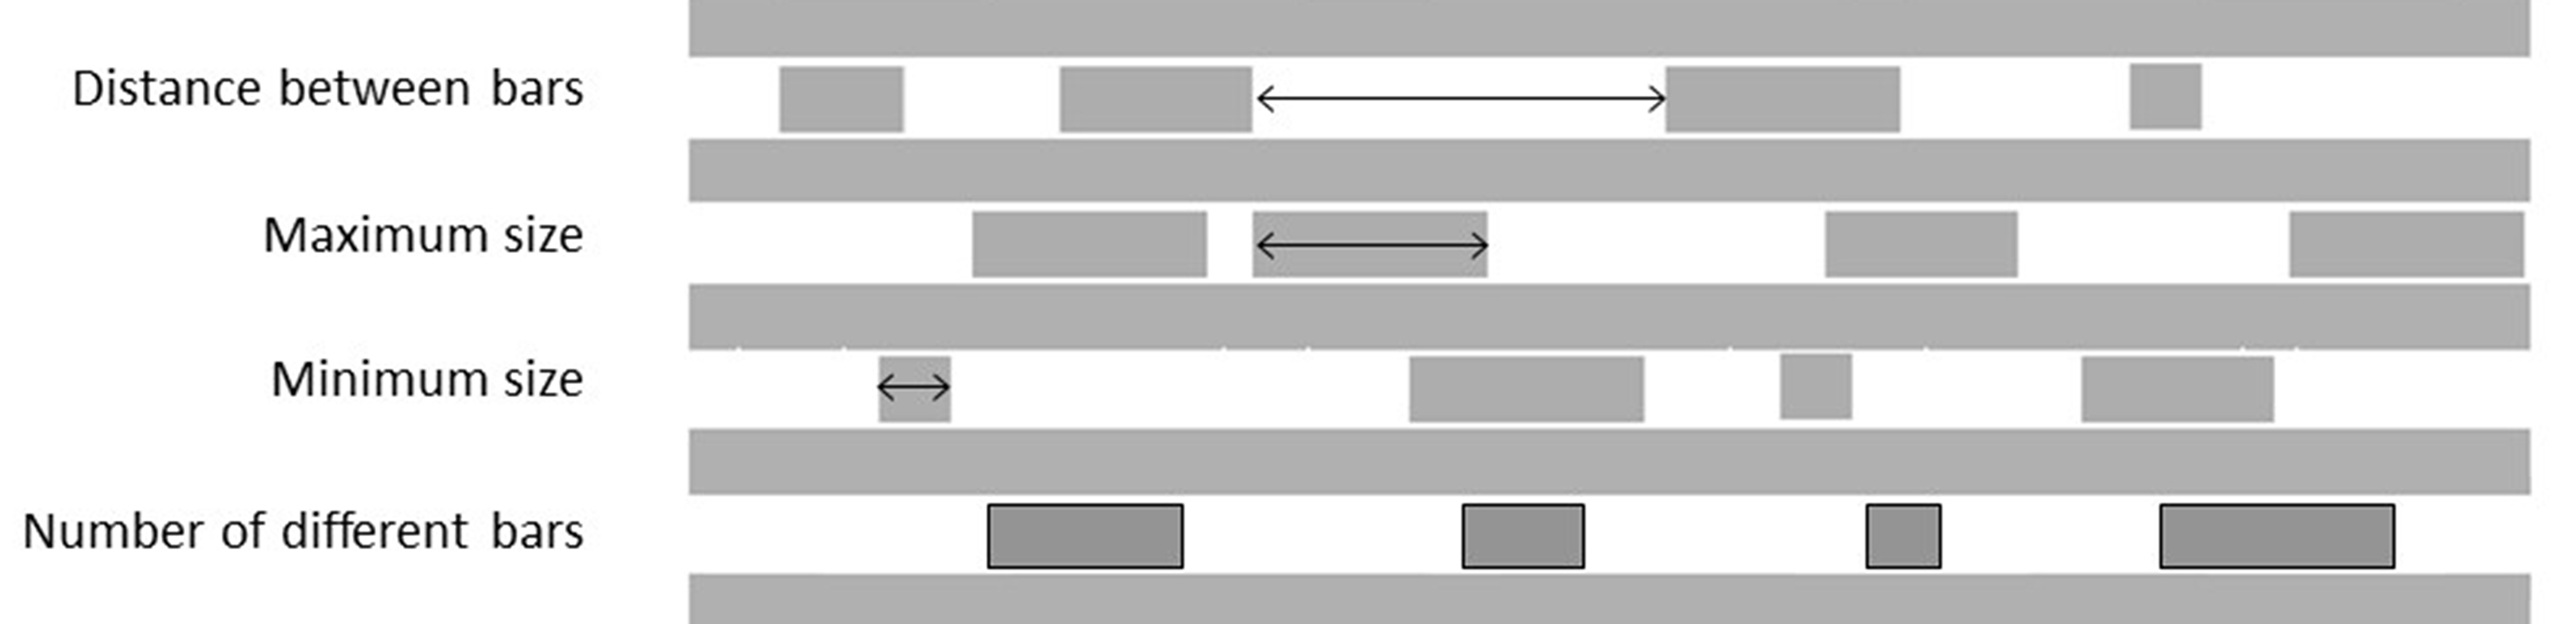
\includegraphics[width=\textwidth]{Images/Evaluation/Ericeira_1.jpg}
	\caption[Ericeira Solarium: Representation of the shading panels' geometric pattern and design variables]{Ericeira Solarium: Representation of the shading panels' geometric pattern and design variables.}
	\label{fig:ericeira_panels_explanation}
\end{figure}

\begin{figure}[htbp]
	\centering
	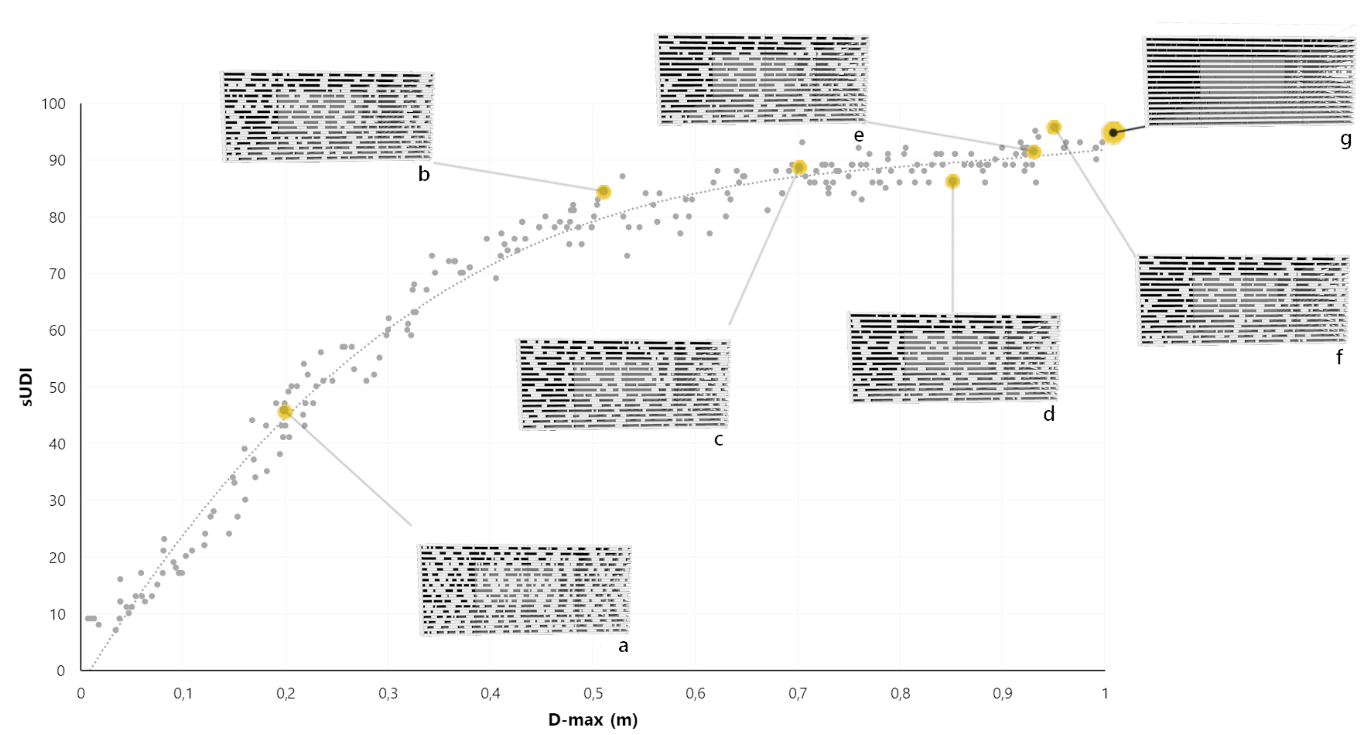
\includegraphics[width=\textwidth]{Images/Evaluation/Ericeira_caadria2018.PNG}
	\caption[Ericeira Solarium: The scatter plot with the samples obtained during the experimental approach]{Ericeira Solarium: The scatter plot with the samples obtained during the experimental approach. The models a. to g. correspond to the set of examples presented to the architects.}
	\label{fig:ericeira_doe}
\end{figure}


\clearpage
\section{Space Frame Optimization}
\label{sec:spaceframeoptimizationextra}

% In the space frame optimization problem, we have evaluated a total of $19$ optimization algorithms. We performed $3$ evaluation runs for each algorithm, each involving $225$ function evaluations. Particularly, for the metaheuristic algorithms, each run comprised a total of $15$ iterations and a total of $15$ solutions per iteration. Conversely, model-based algorithms used the latin hypercube sampling algorithm to sample $100$ initial solutions and create the initial surrogate model, after which the other $125$ evaluations were spent on the evaluation of the best solutions found by the different strategies ($NSGA$-$II$, $Random$, $SMPSO$) during the optimization of the surrogate model.

% Metaheuristics' parameters, such as \textit{population\_size}, \textit{swarm\_size}, \textit{leader\_size}, \textit{max\_iterations}, and \textit{capacity}, i.e., the parameters related to the individuals/particles of each iteration were all set to $15$. Additionally, the \ac{PSO} parameters, \textit{mutation\_probability} and \textit{mutation\_perturbation} were set to $0.3$ and $0.5$, respectively. Since $OMOPSO$ and $\epsilon$-$MOEA$ rely on the Pareto $\epsilon$-dominance concept\footnote{The Pareto $\epsilon$-dominance concept is the same as the Pareto dominance one, but a nondominated solution that lies within a distance $\epsilon$ from other nondominated solution will not be considered as optimal.}, the parameter \textit{epsilons} was set to $[0.1, 0.5]$.

% Regarding the parameters of model-based algorithms: individuals/particle-related parameters were set to $50$ and the number of iterations for each search strategy was set to $10$. All other metaheuristics' parameters were also applied in the search strategies used in the model-based algorithms. The $Random$ strategy was the only exception, as it only required two parameters the \textit{sampling\_function}, which was set to be the Monte Carlo sampling strategy, and the \textit{nsamples}, which was set to $1000$.

\begin{table}[h!]
	\centering
	\label{table:configurationsspaceframe}
	\caption[Space Frame: Hyperparameters of the tested optimization optimization algorithms]{Space Frame: Hyperparameters of the 19 tested optimization algorithms. All others are taken to be the default values available in the optimization libraries.}
	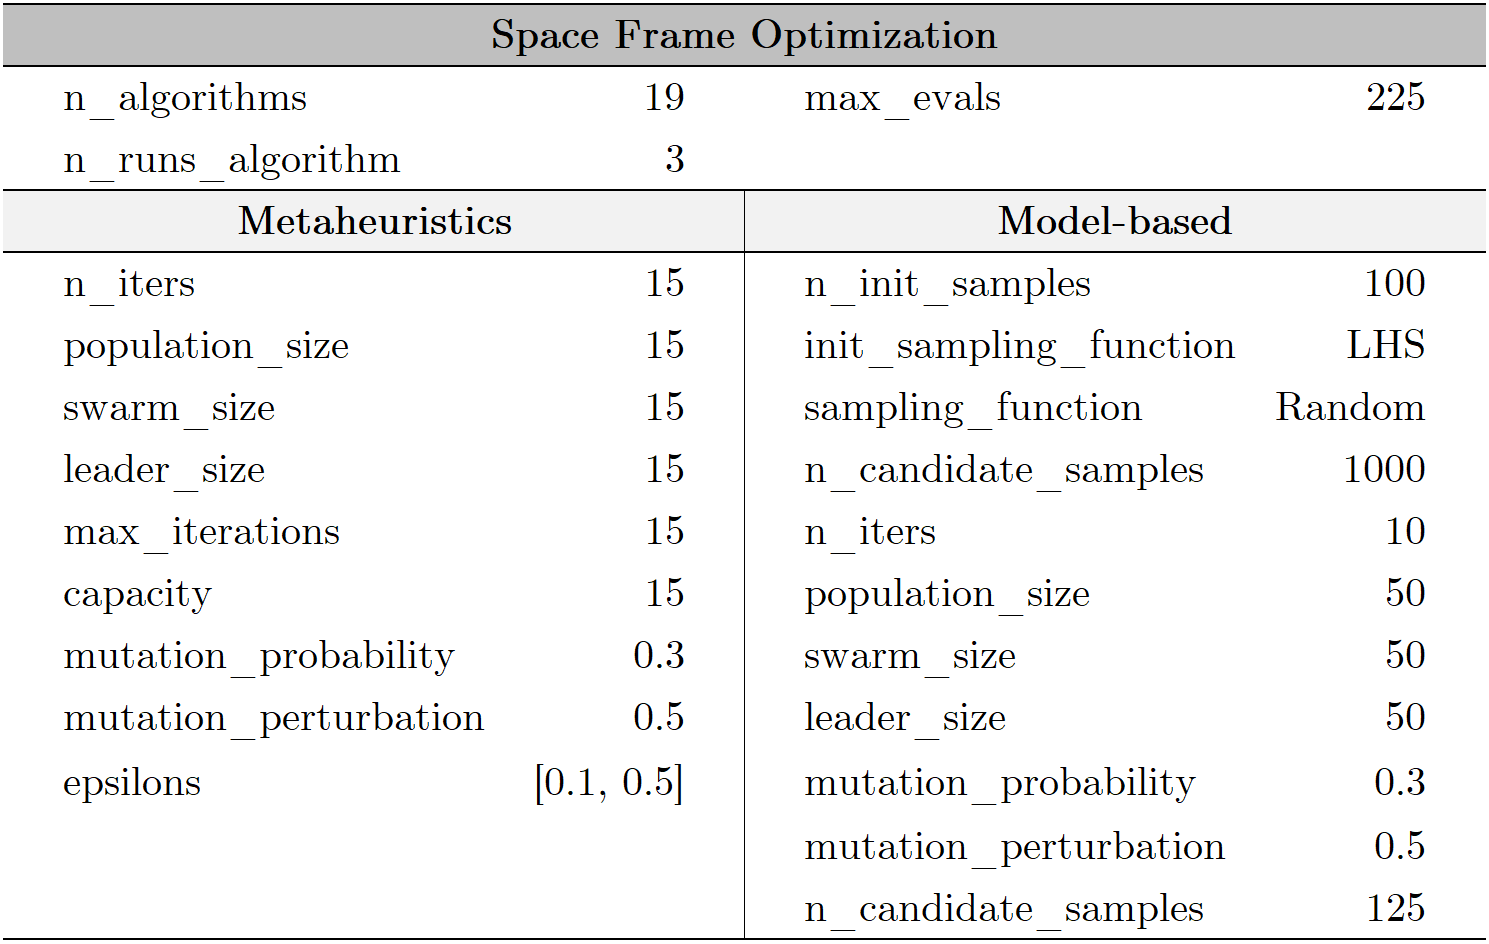
\includegraphics[width=\textwidth]{tables_and_code/appendices/configs_space_frame.PNG}
\end{table}

\begin{figure}[h!]
	\centering
	\includegraphics[width=\textwidth]{Images/Evaluation/caadria/All_Algorithms_run1-2019-04-13.png}
	\caption[Space Frame: Pareto Fronts for run 1]{Space Frame: Algorithms' Pareto fronts for the bi-objective space frame optimization problem. Pareto fronts based on the results of run $1$ and the resulting combined front (black dots).}
	\label{table:spaceframerun1}
\end{figure}

\begin{figure}[h!]
	\centering
	\includegraphics[width=\textwidth]{Images/Evaluation/caadria/All_Algorithms_run2-2019-04-13_1.png}
	\caption[Space Frame: Pareto Fronts for run 2]{Space Frame: Algorithms' Pareto fronts for the bi-objective space frame optimization problem. Pareto fronts based on the results of run $2$ and the resulting combined front (black dots).}
	\label{table:spaceframesrun2}
\end{figure}

\begin{figure}[h!]
	\centering
	\includegraphics[width=\textwidth]{Images/Evaluation/caadria/All_Algorithms_run3-2019-04-13.png}
	\caption[Space Frame: Pareto Fronts for run 3]{Space Frame: Algorithms' Pareto fronts for the bi-objective space frame optimization problem. Pareto fronts based on the results of run $3$ and the resulting combined front (black dots).}
	\label{table:spaceframerun3}
\end{figure}

\clearpage
\section{Black Pavilion: Skylights Optimization}
\label{sec:blackpavilionextra}

% In the black pavilion optimization problem, we have evaluated a total of $10$ optimization algorithms. We performed $3$ evaluation runs for each algorithm, each involving $200$ function evaluations. Particularly, for the metaheuristic algorithms, each run comprised a total of $20$ iterations and a total of $10$ solutions per iteration. Conversely, model-based algorithms used the Monte Carlo sampling algorithm to generate $75$ solutions and create the initial surrogate model, after which the other $125$ evaluations were spent on the evaluation of the best solutions found by the different strategies ($NSGA$-$II$, $SPEA2$, $Random$) during the optimization of the surrogate model.

% Metaheuristics' parameters, such as \textit{population\_size}, \textit{leader\_size}, \textit{max\_iterations}, i.e., the parameters related to the individuals/particles of each iteration were all set to $10$. Additionally, the \ac{PSO} parameters, \textit{mutation\_probability} and \textit{mutation\_perturbation} were set to $0.3$ and $0.5$, respectively. Since $OMOPSO$ relies on the Pareto $\epsilon$-dominance concept, the parameter \textit{epsilons} was set to $[0.5, 100]$.

% Regarding the parameters of model-based algorithms: individuals-related parameters were set to $10$ and the number of iterations for each search strategy was set to $400$. The $Random$ strategy required two parameters: the \textit{sampling\_function}, which was set to be the Monte Carlo sampling strategy, and the \textit{nsamples}, which was set to $400$.

\begin{table}[h!]
	\centering
	\label{table:configurationsspaceframe}
	\caption[Black Pavilion: Hyperparameters of the tested optimization optimization algorithms]{Space Frame: Hyperparameters of the 10 tested optimization algorithms. All others are taken to be the default values available in the optimization libraries.}
	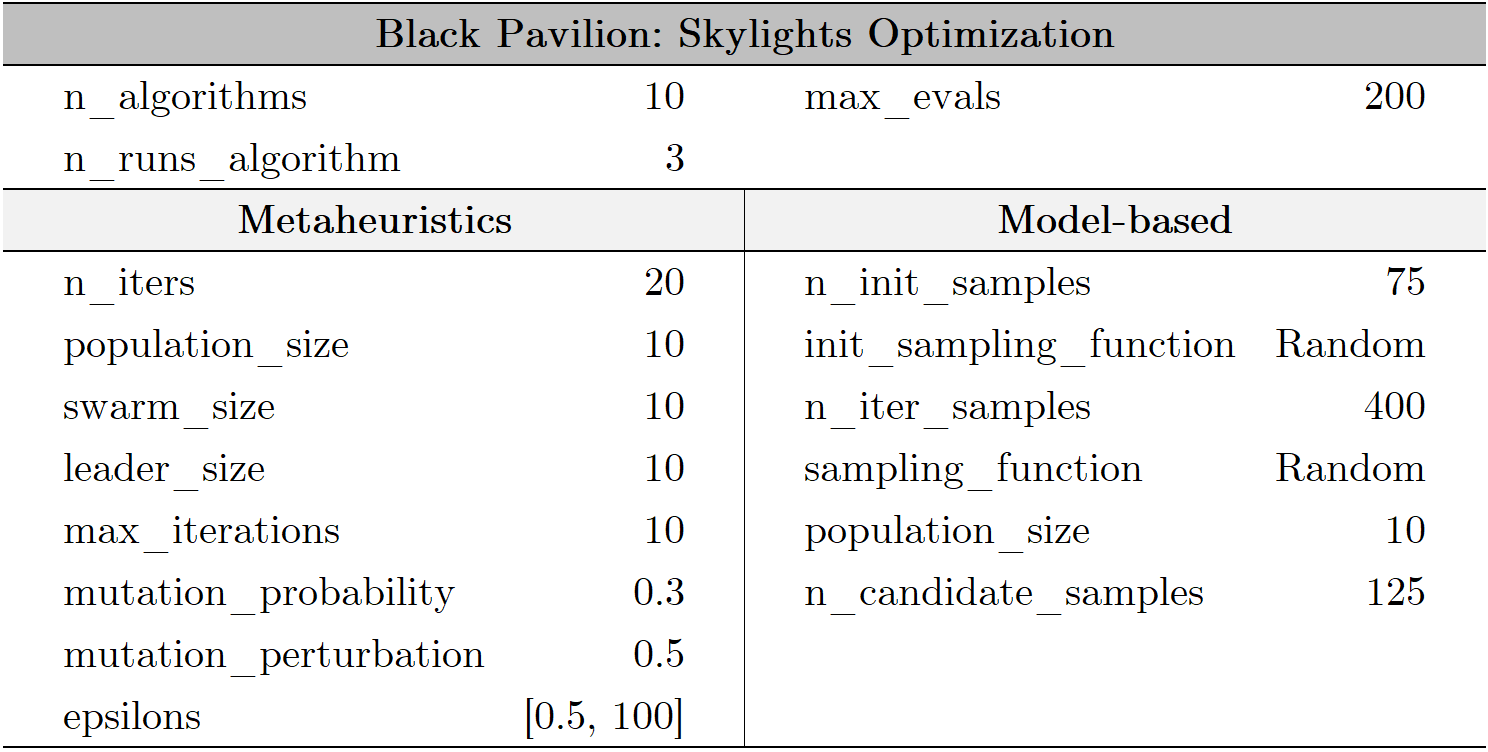
\includegraphics[width=\textwidth]{tables_and_code/appendices/configs_black_pavilion.PNG}
\end{table}


\begin{figure}[h!]
	\centering
	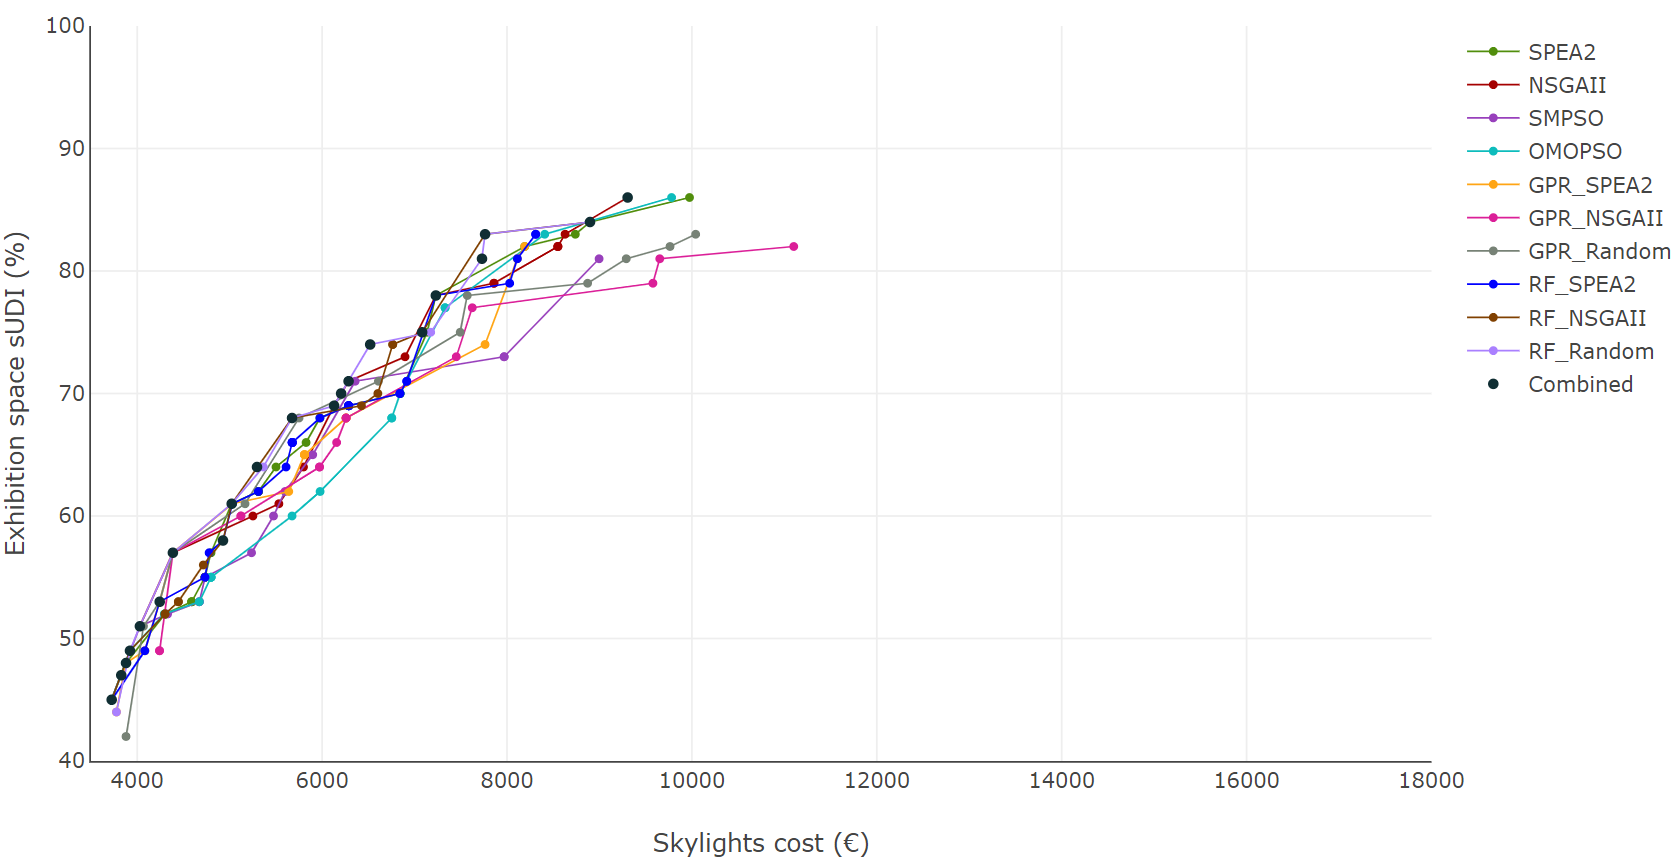
\includegraphics[width=\textwidth]{Images/Evaluation/BlackPavilion/All_Algorithms_run1-2019-04-19.png}
	\caption[Black Pavilion: Pareto Fronts for run 1]{Black Pavilion: Algorithms' Pareto fronts for the bi-objective black pavilion optimization problem. Pareto fronts based on the results of run $1$ and the resulting combined front (black dots).}
	\label{table:blackpavilionrun1}
\end{figure}

\begin{figure}[h!]
	\centering
	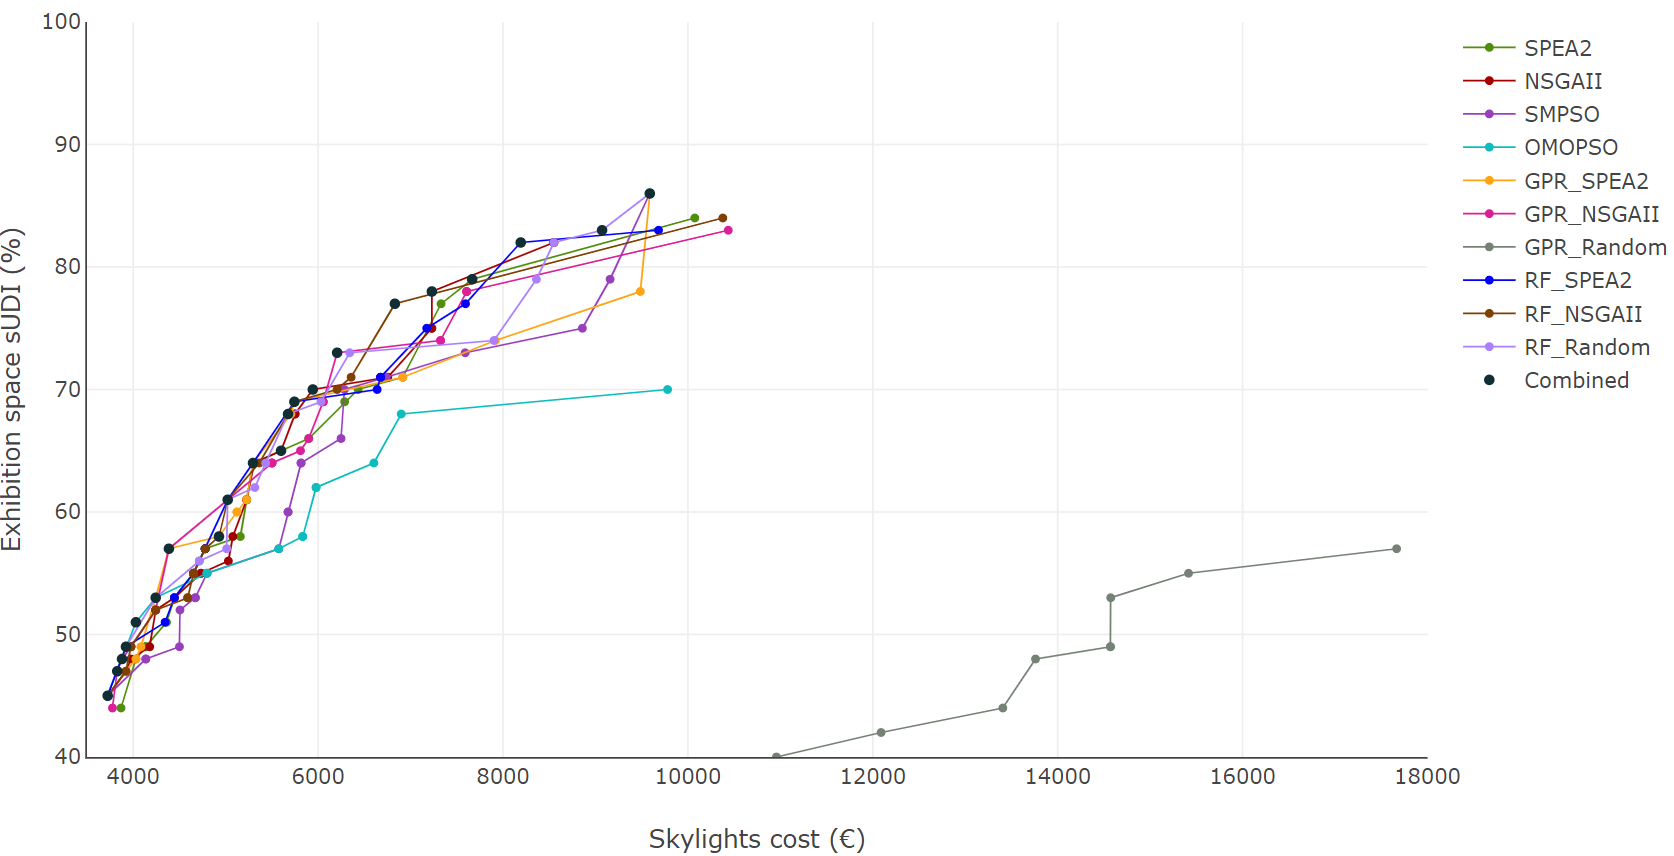
\includegraphics[width=\textwidth]{Images/Evaluation/BlackPavilion/All_Algorithms_run2-2019-04-19.png}
	\caption[Black Pavilion: Pareto Fronts for run 2]{Black Pavilion: Algorithms' Pareto fronts for the bi-objective bolack pavilion optimization problem. Pareto fronts based on the results of run $2$ and the resulting combined front (black dots).}
	\label{table:blackpavilionrun2}
\end{figure}

\begin{figure}[h!]
	\centering
	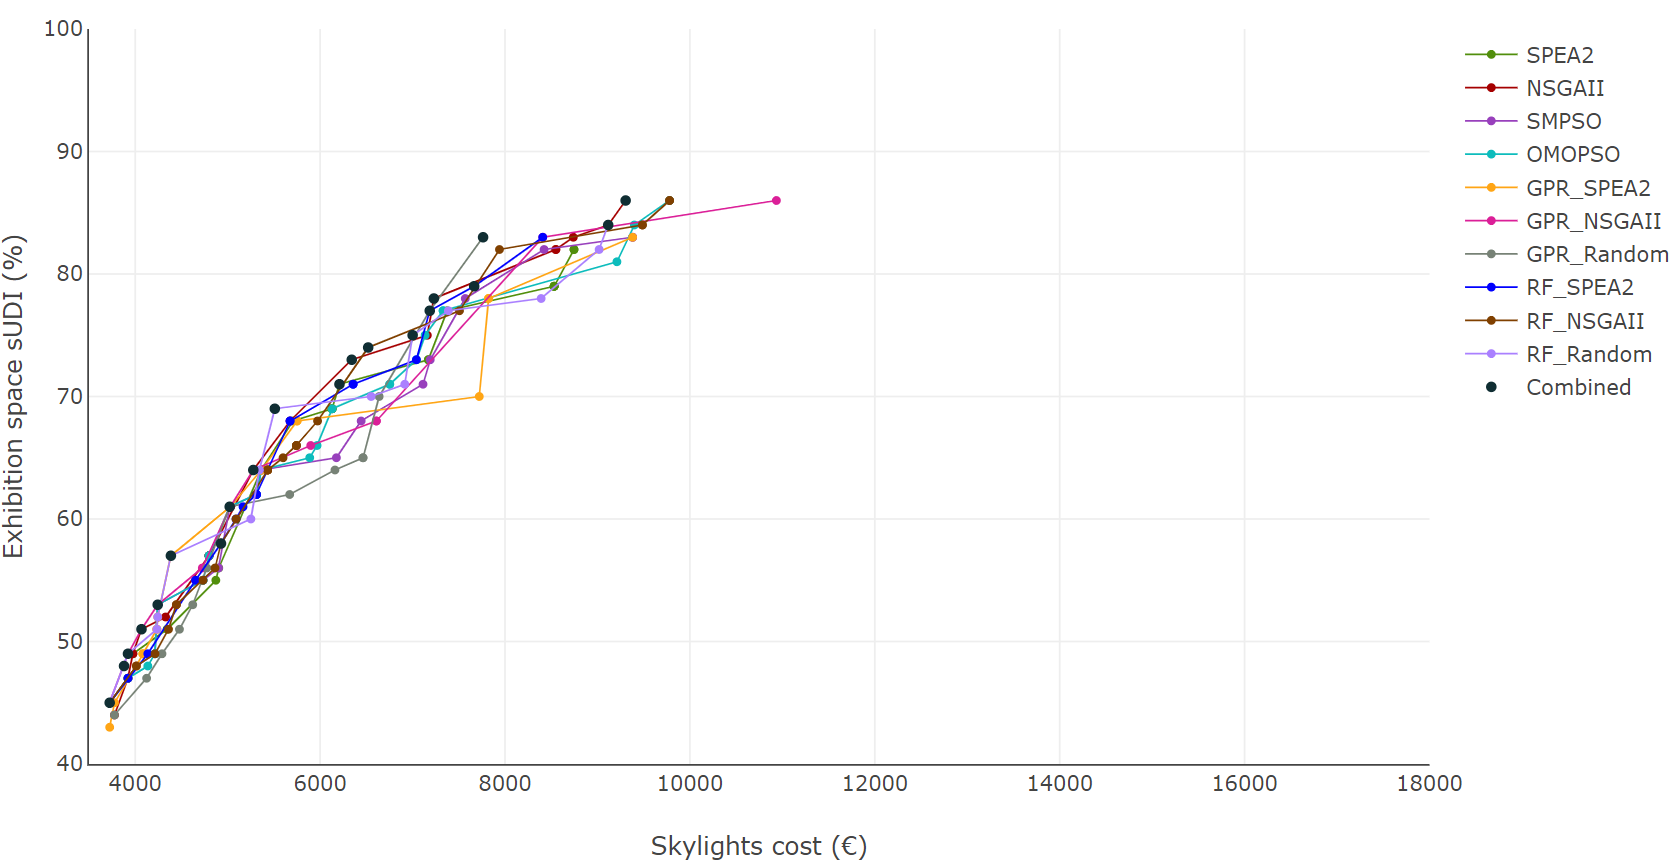
\includegraphics[width=\textwidth]{Images/Evaluation/BlackPavilion/All_Algorithms_run3-2019-04-19_2.png}
	\caption[Black Pavilion: Pareto Fronts for run 3]{Black Pavilion: Algorithms' Pareto fronts for the bi-objective black pavilion optimization problem. Pareto fronts based on the results of run $3$ and the resulting combined front (black dots).}
	\label{table:blackpavilionrun3}
\end{figure}
